\documentclass[11pt]{jsarticle}%article??

\usepackage{../mypackage}
%\usepackage[top=10truemm,bottom=10truemm,left=15truemm,right=15truemm]{geometry}
\usepackage[]{multicol}

\usepackage{titlesec}

\titleformat*{\section}{\large\bfseries}
\titleformat*{\subsection}{\normalsize\bfseries}

%
% ######## measure #########
% # mm = 1mm = 2.85pt      #
% # cm = 10mm = 28.5pt     #
% # in = 25.4mm = 72.27pt  #
% # pt = 0.35mm = 1pt      #
% # em = width of [M]      #
% # ex = height of [x]     #
% # zw = width of [Kanji]  #
% # zh = height of [Kanji] #
% ##########################
% ##################### Portrait Setting #########################
% # TOP = 1inch + ¥voffset + ¥topmargin + ¥headheight + ¥headsep #
% #     = 1inch + 0pt + 4pt + 20pt + 18pt (default)              #
% # BOTTOM = ¥paperheight - TOP -¥textheight                     #
% ################################################################
\setlength{\textheight}{\paperheight}   % 紙面縦幅を本文領域にする(BOTTOM=-TOP)
\setlength{\topmargin}{-5.4truemm}       % 上の余白を30mm(=1inch+4.6mm)に
\addtolength{\topmargin}{-\headheight}  % 
\addtolength{\topmargin}{-\headsep}     % ヘッダの分だけ本文領域を移動させる
\addtolength{\textheight}{-40truemm}    % 下の余白も30mm(BOTTOM=-TOPだから+TOP+30mm)
% #################### Landscape Setting #######################
% # LEFT = 1inch + ¥hoffset + ¥oddsidemargin (¥evensidemargin) #
% #      = 1inch + 0pt + 0pt                                   #
% # RIGHT = ¥paperwidth - LEFT - ¥textwidth                    #
% ##############################################################
\setlength{\textwidth}{\paperwidth}     % 紙面横幅を本文領域にする(RIGHT=-LEFT)
\setlength{\oddsidemargin}{-15.4truemm}  % 左の余白を25mm(=1inch-0.4mm)に
\setlength{\evensidemargin}{-15.4truemm} % 
\addtolength{\textwidth}{-25truemm}     % 右の余白も25mm(RIGHT=-LEFT)
%
%

\newif\iffigure
%\figurefaulse
\figuretrue
%select show the figure or not

\makeatletter
\def\@cite#1{\textsuperscript{#1)}}
\def\@biblabel#1{#1)}
\makeatother

\newcommand{\DATE}[3]{#1年#2月#3日} 
\newcommand{\TheDay}{\DATE{2020}{12}{01}}
\newcommand{\rHeader}{東京大学工学部航空宇宙工学科 中須賀・船瀬研究室}
\newcommand{\lHeader}{令和2年度学士論文}

%題名は重要そう
\title{コマンドを用いた衛星の不具合分析支援に関する研究} 
\date{\TheDay} %これ日付と名前が横配置にできないかを考える
\author{03-183005 西本 慎吾}

%ヘッダの指定:
\pagestyle{fancy}

\begin{document}
%2段組みにする
\maketitle

%ここら辺のフォントを変えたい
\thispagestyle{fancy}
\lhead[\lHeader]{\lHeader} % ヘッダ左側
%\chead[偶数ページの引数]{奇数ページの引数} %ヘッダ中央
\rhead[\rHeader]{\rHeader} %ヘッダ右側
%\lfoot[偶数ページの引数]{奇数ページの引数} %フッタ左側
%\cfoot[偶数ページの引数]{奇数ページの引数} %フッタ中央
%\rfoot[偶数ページの引数]{奇数ページの引数} %フッタ右側

%\columnseprule=0.3mm

\begin{abstract}
  近年,大学や高専などの教育機関や,民間企業による超小型衛星の
開発,およびそれを利用した事業の展開が盛んになっている.
一方で,超小型衛星の信頼性の低さが問題となっている.%修正
信頼性の低さの原因として,設計および製造過程における不良が多いことが分かっており,
地上試験によって不具合の改修,対策を十分に行うことが重要である.
 しかし,衛星のような複雑なシステムでは,内部の機器間で異常状態が%これおかしい
波及するため,不具合事象から
故障箇所の特定を行うことは非常に多くの知識と経験を必要とする. 
 そこで,本研究ではコンポーネント間の接続関係モデル,情報
 伝達の経路モデルを用いて衛星の故障候補の
 検証方法(確認事項,打つべきコマンド)を人間の判断を支援する
 指標と共に提示することで,不具合分析を支援する手法を提案する.
 本手法では,簡易的な衛星モデルに対して実践することで
 コマンドによる故障箇所の特定を効率的に行えること,設計の不備を発見
することにつながることを確認した.
%多分背景以外のところをもう少し詳細に述べたほうがいい気がする.
\end{abstract}

\begin{multicols}{2}
  \section{序論}
  \vspace{-1zh}
  \subsection{研究背景}
  \vspace{-1zh}
  超小型衛星の信頼性の低さ,それを解決するためには設計製造過程に
  おける信頼性を上げる必要がある.
  設計・製造における不良が軌道上故障の多くを占めている現状がある.
  解決するためには地上試験において,設計上の不良を発見し十分に改修しなけらばならない.

  \begin{figure}[H]
    \centering
      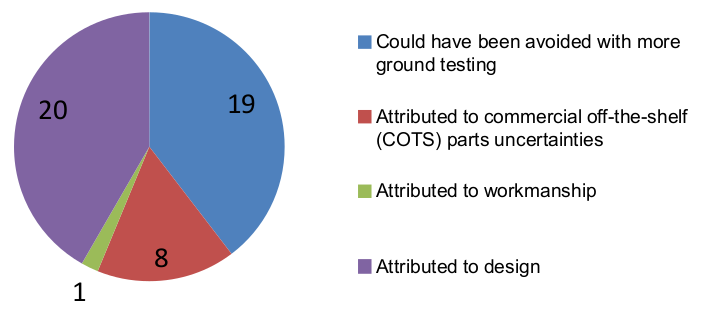
\includegraphics[height=3.0cm]{../figure/cause_of_failure.png}
      \caption{超小型衛星の故障原因に関する調査結果\cite{Venturini2017}}
      \label{fig:cause_of_failure}
  \end{figure}
  
 % \vspace{-1zh}
  %地上試験の不備が発生する原因として地上試験で改修を行う難しさがあるということを言いたい
  \subsection{問題提起}
  \vspace{-1zh}
  以上より,地上試験での不具合分析が不十分になっていることが,超小型衛星の
  信頼性の低さの原因の一つである.地上試験での不具合分析を十分に行うためには
  以下の2点の作業に高い知識と経験が必要とされる.
  \begin{itemize}
    \item 故障候補の網羅的洗い出し
    \item 故障候補の切り分け作業
  \end{itemize}
%故障仮説の網羅的洗い出市に関する研究についてもう少しまとめる
これに対して,下表\ref{tab:previous_research}に示すように,
故障候補の洗い出しを網羅的に行う研究が盛んにおこなわれている.
故障仮説を網羅的に生成するために,物理現象を表現するオントロジーを考案し,故障原因の
粒度まで切り分けて仮説の生成を可能にしている.
一方で,故障候補の切り分ける過程に関して取り組んだ研究は少ない.
%安全に行う必要があることを言いたい.

\vspace{-1zh}
%比較軸が微妙過ぎる
\begin{table}[H]
  \centering
  \caption{不具合分析手法の比較}
  \label{tab:previous_research}
   \scalebox{0.9}{
     \begin{tabular}{cccccc} \hline%もう少し示し方を考える.
        手法&故障網羅性&手法の目的%&モデル複雑度%専門家の知識が必要という点で?
        \\ \hline
        GDE&低&故障仮説生成%&低
        \\ %見てないし無くてもいいかも
        GDE+\cite{Struss1989}&中&故障仮説生成%&中
        \\
        網状故障解析\cite{Yamaguchi2014}&中&異常モード洗い出し%&高
        \\
        故障オントロジー\cite{Kitamura1999}&高&故障仮説生成%&高
        \\
        本手法&中%低かもしれない.接続関係しか見れていない
        &故障箇所特定%&中
        \\ \hline
     \end{tabular}}
\end{table}
\vspace{-1zh}
\subsection{本研究の目的}
  以上より,次の機能を持った不具合事象から故障候補の切り分けまでの作業を支援する手法を提案する.
%コマンドとテレメトリをベースにしたものを対象にしていることを言った方がいいかもしれない
  \begin{itemize}
  \item 異常テレメトリから,故障候補を生成する
  \item 故障候補を確認するためのコマンドおよびテレメトリを探索する.
  \item 上の探索結果に関して優先度を人間に提示する.
\end{itemize}
したがって,上記の機能を達成するために以下の3点の構築を目的とする.%???
\begin{itemize}
  \item 衛星内部機器の接続関係モデル及び情報伝達経路モデル
  \item 故障箇所の特定を行うために必要なコマンド及びテレメトリの探索
  \item 人間の判断を支援するコマンドの評価指標の提案
\end{itemize}
\vspace{-1zh}
\section{モデルベース不具合分析手法の仕様}
\vspace{-1zh}
\subsection{不具合分析アルゴリズム}
\vspace{-1zh}
人と対話的に故障箇所を絞り込んでいく手法になっているため,人による
不具合分析の流れを下図\ref{fig:fault_diagnosis_flow}に示す.
%ちょっと文字が小さい
\begin{figure}[H]
  \centering
    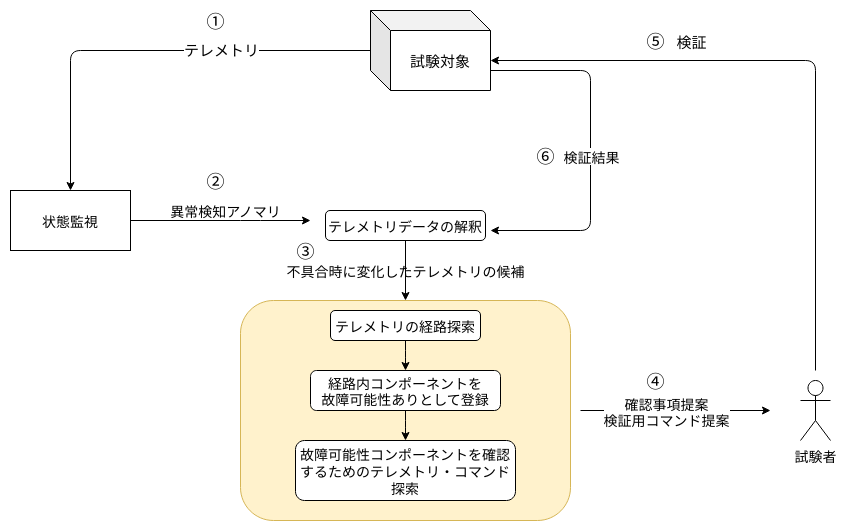
\includegraphics[height=5.5cm]{../figure/fault_diagnosis_flow.png}
    \caption{本手法による不具合分析の流れ}
    \label{fig:fault_diagnosis_flow}
\end{figure}

\subsection{モデル}%オントロジーやけどね
本手法で使用するモデルをいかに示す.

  コンポーネント間接続関係モデル.
  情報伝達経路モデル
  コマンドおよびテレメトリの機能モデル%これは違うかも

  \subsection{評価指標の提案}
  探索を行った結果を提示し,人間が選択する際に必要となる指標を
  以下の2点に分けて示す.
  \begin{itemize}
    \item 衛星の生存性への副作用
    \item 故障候補切り分け能力の大きさ
  \end{itemize}

  \subsubsection{衛星の生存への副作用}
  まず,生存への副作用を示す指標として,以下の3点を与える.
  \begin{itemize}
    \item コマンドを打つ前の電力状態と,コマンドを打つことによって発生する電力消費量
    \item 姿勢変化を起こすか否か
    \item コマンド送信によって変化するテレメトリの数
  \end{itemize}

  \subsubsection{故障候補切り分け能力}

  %これも文字小さい.この図で説明する必要があるのか?
  \begin{figure}[H]
    \centering
       \begin{tabular}{c}
          \begin{minipage}{0.30\hsize}
          \centering
          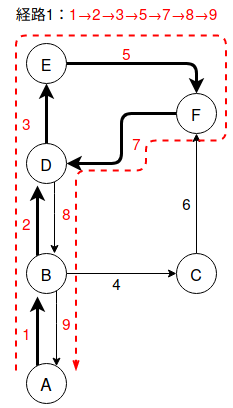
\includegraphics[height=4cm]{../figure/route1.png}
           %  \caption{}
             \label{fig:route1}
          \end{minipage}
          \begin{minipage}{0.30\hsize}
          \centering
          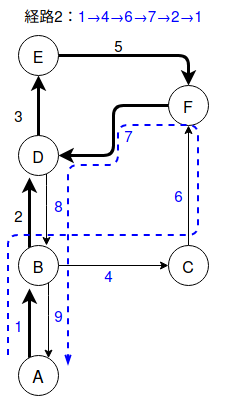
\includegraphics[height=4cm]{../figure/route2.png}
          %\caption{}
             \label{fig:route2}
          \end{minipage}
          \begin{minipage}{0.30\hsize}
             \centering
             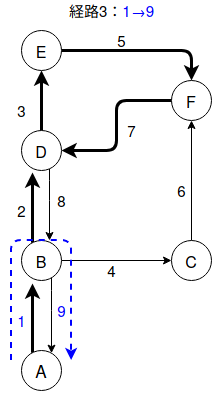
\includegraphics[height=4cm]{../figure/route3.png}
             %\caption{}
                \label{fig:route2}
             \end{minipage}
       \end{tabular} 
       \caption{故障候補とそれを確認するための情報伝達経路の例}%ここも変えたほうがいいかも
       \label{fig:route}
 \end{figure}
故障候補を確認するためには経路内に存在する他のリンクが正常である必要がある.
その制約によって,確認するための確率を求めることが可能である.

  対象のコマンドから分析をスタートした時に,最終的に故障個所の特定を行うまでの
  総コマンド数の期待値が求められる.
  各リンクに対して正常確率を用いることで,テレメトリが正常になるかどうかの確率を計算し,それらの結果に基づく
  次のコマンドの探索に移る.
  %ココらへんのアルゴリズムを分かりやすく示すための図が欲しいかもしれない
  結果による分岐状態を図示する?木構造になるため
  データとして扱いにくいことこの上ない.

  \subsubsection{故障候補切り分け能力}

  %書くべき事項
  確認可能性に関する説明.それをもとに確認の順序を考えていく必要があるということ
  確認結果による条件分岐が発生し,それに応じた結果によって次のコマンドが変化すること.など
  


  地上試験と軌道上運用における使い分け

  \section{提案手法による実践と評価}
  \subsection{対象問題設定と実践結果}
  実践例での対象故障.
  複数の事例を確認して,どうだったかという結果も欲しい

  \subsection{}

  \section{結論}
  \subsection{本研究で得られた知見}
  
  \subsection{今後の展望}

  故障候補の網羅的な生成を実現するために,先行研究で取り組まれている
  オントロジーを作り,..

  ある程度の事前定義情報からモデル化を自動化することを目標にする.
  


  
  \bibliographystyle{junsrt} %plain, acm, alpha とか
  \bibliography{../Ref} 

\end{multicols}
\end{document}